\documentclass{article}

\usepackage[margin=.44 in]{geometry}
\usepackage{amsmath,amsfonts,textcomp,amssymb,amscd,amsthm,mathrsfs,mathtools}
\usepackage{graphicx,tikz}
\usetikzlibrary{matrix,calc,arrows.meta,angles,quotes,positioning,shapes,fit,backgrounds}
\usepackage{hhline,xcolor}
\usepackage{pgfplots}
\usepackage{lipsum}
\usepackage[mathscr]{euscript}
\usepackage{tcolorbox}
\tcbuselibrary{hooks, breakable, skins}
\pgfplotsset{compat=1.11}

\newsavebox{\boxedalignbox}
\newenvironment{boxedalign*}
{\begin{equation*}\begin{lrbox}{\boxedalignbox}$\begin{aligned}}
			{\end{aligned}$\end{lrbox}\fbox{\usebox{\boxedalignbox}}\end{equation*}}
		
\newcommand*{\colorboxed}{}
\def\colorboxed#1#{%
	\colorboxedAux{#1}%
}
\newcommand*{\colorboxedAux}[3]{%
	% #1: optional argument for color model
	% #2: color specification
	% #3: formula
	\begingroup
	\colorlet{cb@saved}{.}%
	\color#1{#2}%
	\boxed{%
		\color{cb@saved}%
		#3%
	}%
	\endgroup
}

\setlength{\parindent}{0pt}
\setlength{\parskip}{1em}

\DeclareSymbolFont{rsfs}{U}{rsfs}{m}{n}
\DeclareSymbolFontAlphabet{\mathscrsfs}{rsfs}

\makeatletter

\newcommand*\curveplus{%
	\mathbin{\rotatebox[origin=c]{90}{$\m@th\curvearrowleft$}+}}

\newcommand*\rightplus{%
	\mathpalette\@rightplus\relax}
\newcommand*\@rightplus[1]{%
	\mathbin{\vcenter{\hbox{$\m@th\overset{#1+}{\to}$}}}}

\newcommand*\upplus{%
	\mathbin{+\mathord\uparrow}}


\title{Tensor}
\author{Md. Mesbahose Salekeen}
\date{}

\begin{document}
	
	\maketitle
	\large
	\section*{Tensor}
	1.In basic terms tensor can be called a multidimensional array of numbers. For example,
	\begin{figure}[hbp]
		\begin{center}
			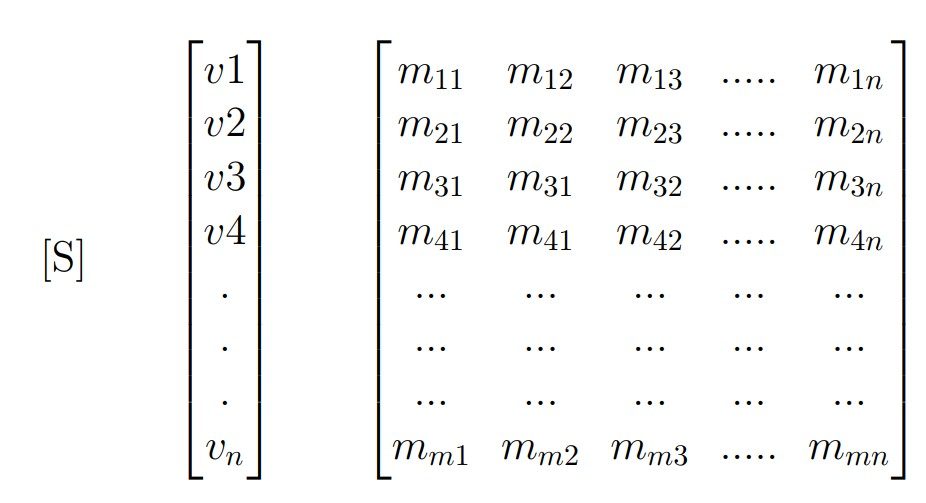
\includegraphics[scale=0.35]{1.jpg}
			\label{f1}
		\end{center}
	\end{figure}

	\begin{center}
	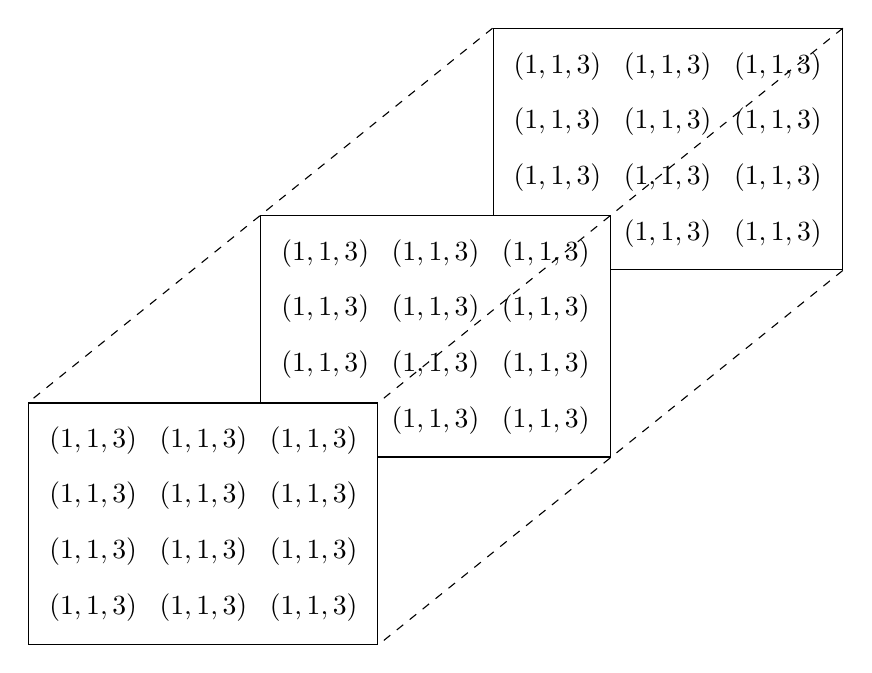
\begin{tikzpicture}[every node/.style={anchor=north east,fill=white,minimum width=1.4cm,minimum height=7mm}]
		\matrix (mA) [draw,matrix of math nodes]
		{
			(1,1,3) & (1,1,3) & (1,1,3) \\
			(1,1,3) & (1,1,3) & (1,1,3) \\
			(1,1,3) & (1,1,3) & (1,1,3) \\
			(1,1,3) & (1,1,3) & (1,1,3) \\
		};
		
		\matrix (mB) [draw,matrix of math nodes] at ($(mA.south west)+(1.5,0.7)$)
		{
			(1,1,3) & (1,1,3) & (1,1,3) \\
			(1,1,3) & (1,1,3) & (1,1,3) \\
			(1,1,3) & (1,1,3) & (1,1,3) \\
			(1,1,3) & (1,1,3) & (1,1,3) \\
		};
		
		\matrix (mC) [draw,matrix of math nodes] at ($(mB.south west)+(1.5,0.7)$)
		{
			(1,1,3) & (1,1,3) & (1,1,3) \\
			(1,1,3) & (1,1,3) & (1,1,3) \\
			(1,1,3) & (1,1,3) & (1,1,3) \\
			(1,1,3) & (1,1,3) & (1,1,3) \\
		};
		
		\draw[dashed](mA.north east)--(mC.north east);
		\draw[dashed](mA.north west)--(mC.north west);
		\draw[dashed](mA.south east)--(mC.south east);
	\end{tikzpicture}
	\end{center}

	2. But this is not a clear definition of tensor. Of course we can represent tensors as
	arrays but that’s does not give the whole picture. One better definition is:
	Tensor is an object that is invariant under a change of co-ordinates system
	and has components that change in a special and predictable way under a
	change of co-ordinates system
	
	3. A collection of vectors and covectors combined together using tensor product.(Tensor
	can be understood as partial derivative and gradient that transforms with jacobian matrix)
	
	\section*{Coordinate Transformation}
	\begin{figure}[hbp]
		\begin{center}
			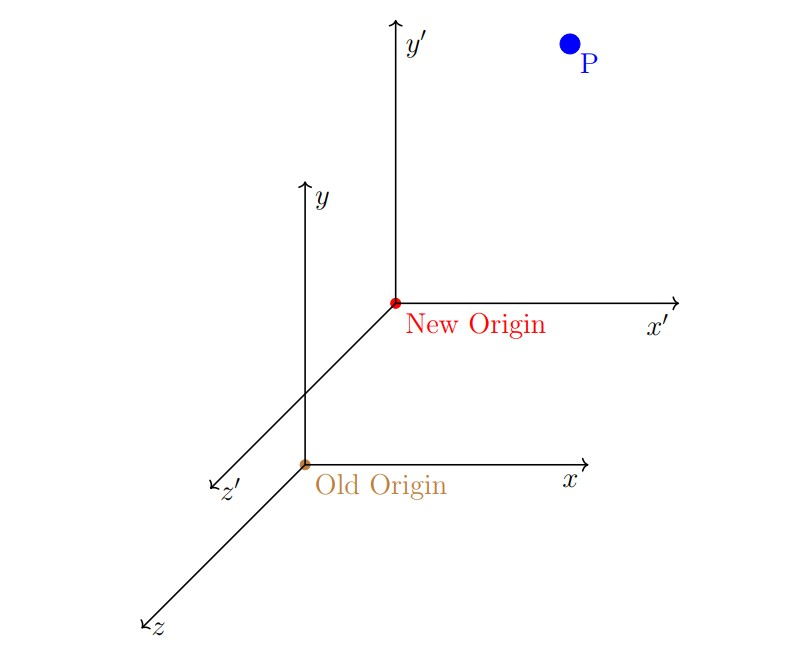
\includegraphics[scale=0.45]{2.jpg}
			\label{f2}
		\end{center}
	\end{figure}	
	
	Now let us declare three unit vector $\overrightarrow{e_{1}},\overrightarrow{e_{2}},\overrightarrow{e_{3}}$ in the current/old basis and three unit vector $\widetilde{\overrightarrow{e_{1}}},\widetilde{\overrightarrow{e_{2}}},\widetilde{\overrightarrow{e_{3}}}$
	
	Trying to express new unit vector in terms of old gives us
	\begin{tcolorbox}
		\begin{equation}
			\begin{split}
				\widetilde{\overrightarrow{e_{1}}} &= F_{1}^{1}\overrightarrow{e_{1}} + F_{2}^{1}\overrightarrow{e_{2}} + F_{3}^{1}\overrightarrow{e_{3}}\\
				\widetilde{\overrightarrow{e_{2}}} &= F_{2}^{1}\overrightarrow{e_{1}} + F_{2}^{2}\overrightarrow{e_{2}} + F_{2}^{3}\overrightarrow{e_{3}}\\
				\widetilde{\overrightarrow{e_{3}}} &= F_{3}^{1}\overrightarrow{e_{1}} + F_{3}^{2}\overrightarrow{e_{2}} + F_{3}^{3}\overrightarrow{e_{3}}
			\end{split} \label{eq1} %\tag{1}
		\end{equation}
	\end{tcolorbox}
	

	Defining, $\overrightarrow{F} = \begin{Bmatrix}
		F_{1}^{1}	& F_{2}^{1} & F_{3}^{1}\\
		F_{1}^{2}	& F_{2}^{2} & F_{3}^{2}\\
		F_{1}^{3}	& F_{2}^{3} & F_{3}^{3}\\
	\end{Bmatrix}$ a forward matrix that transforms old basis to new basis.
	
	We can also get the reverse relation,
	
	\begin{tcolorbox}
		\begin{equation}
			\begin{split}
				\widetilde{\overrightarrow{e_{1}}} &= B_{1}^{1}\overrightarrow{e_{1}} + B_{2}^{1}\overrightarrow{e_{2}} + B_{3}^{1}\overrightarrow{e_{3}}\\
				\widetilde{\overrightarrow{e_{2}}} &= B_{2}^{1}\overrightarrow{e_{1}} + B_{2}^{2}\overrightarrow{e_{2}} + B_{2}^{3}\overrightarrow{e_{3}}\\
				\widetilde{\overrightarrow{e_{3}}} &= B_{3}^{1}\overrightarrow{e_{1}} + B_{3}^{2}\overrightarrow{e_{2}} + B_{3}^{3}\overrightarrow{e_{3}}
			\end{split} \label{eq2}
		\end{equation}
	\end{tcolorbox}
	
	
	Similarly We call, $\overrightarrow{B} = \begin{Bmatrix}
		B_{1}^{1}	& B_{2}^{1} & B_{3}^{1}\\
		B_{1}^{2}	& B_{2}^{2} & B_{3}^{2}\\
		B_{1}^{3}	& B_{2}^{3} & B_{3}^{3}\\
	\end{Bmatrix}$ a backward matrix that transform new basis to old basis

	To sum up, 
		
		\begin{tcolorbox}
			\begin{equation}
				\begin{split}
					\widetilde{\overrightarrow{e_{i}}} &= F_{i}^{j}\overrightarrow{e_{j}}\\
					\overrightarrow{e_{i}} &= B_{i}^{j}\widetilde{\overrightarrow{e_{j}}}
				\end{split}\label{eq3}
			\end{equation}
		\end{tcolorbox}
	
	from equation(\ref{eq3}) we get $$\widetilde{\overrightarrow{e_{i}}} = F_{i}^{j}\overrightarrow{e_{j}} = F_{i}^{j}B_{j}^{k}\widetilde{\overrightarrow{e_{k}}}$$
	
	Equating both sides, when $i = k$ the value will need to be 1 or when $i \neq k$ the value will be 0.
	
	Thus $$\delta^{k}_{i} = F_{i}^{j}B_{j}^{k}$$
	
	\begin{tcolorbox}
		\begin{center}
			\begin{equation}
				\delta_{k}^{i} = \begin{cases}
					1 & i = k \\
					0 & i \neq k 
				\end{cases}\label{eq4}
			\end{equation} 
		\end{center}
	\end{tcolorbox}	

	\section*{Vector}
	Vector is an example of Tensor.
	
	\begin{enumerate}
		\item Vector can be expressed as a list of numbers.
		$$\overrightarrow{v} = \begin{bmatrix}
			v^{1}\\
			v^{2}\\
			v^{3}\\
			..\\
			..\\
			v^{n}
		\end{bmatrix} \quad\quad\quad \overrightarrow{w} = \begin{bmatrix}
		w^{1}\\
		w^{2}\\
		w^{3}\\
		..\\
		..\\
		w^{n}
	\end{bmatrix}$$
	
		\item Vector is an arrow which has geometrical meaning; a value and a direction
		\begin{figure}[hbp]
			\begin{center}
				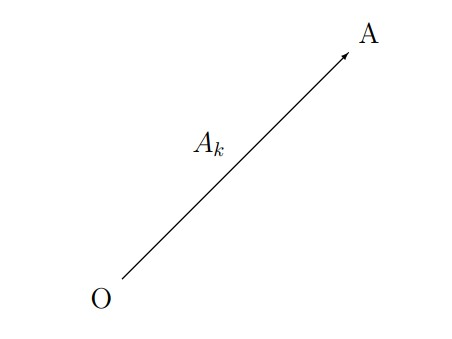
\includegraphics[scale=0.45]{3.jpg}
				\label{f3}
			\end{center}
		\end{figure}
		
		But not all vectors can be represented using arrows and has physical meaning
		
		\item A member of vector space.
			
		\textbf{Vector Space(linear space)} : A vector space (also called a linear space) is a set of objects called vectors,
		which may be added together and multiplied (“scaled”) by numbers called scalars and the result will also
		be a part of that set.
	\end{enumerate}

	\textbf{Field} : In mathematics, a field is a set on which addition, subtraction, multiplication,
	and division are defined and behave as the corresponding operations on rational and real
	numbers do.
	
	\textbf{Cartesian Product} : In mathematics, specifically set theory, the cartesian product of two
	sets A and B, denoted $A \times B$, is the set of all ordered pairs (a, b) where a is in A and b
	is in B. In mathematical terms,
	
	$$A\times B = (a,b) | a\in A \text{ and } a\in B$$
	\begin{figure}[hbp]
		\begin{center}
			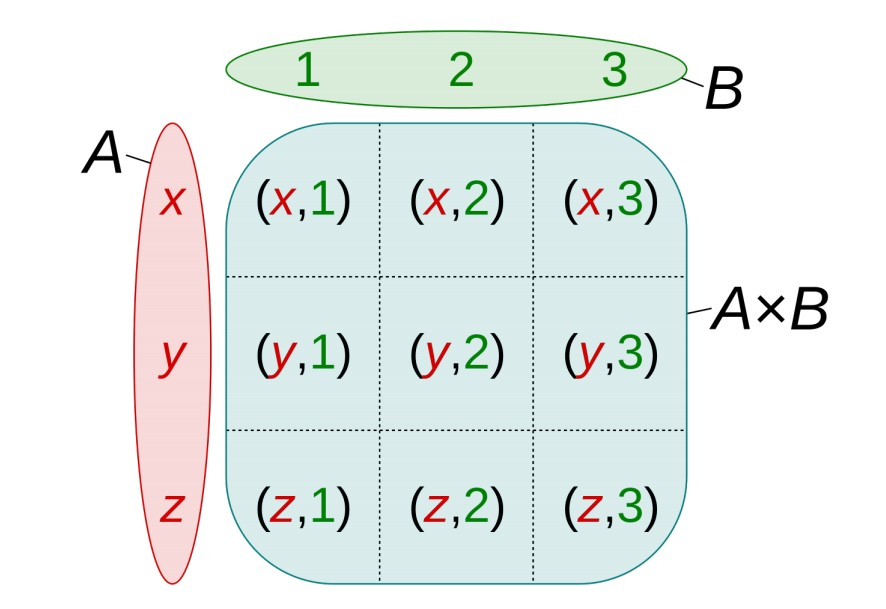
\includegraphics[scale=0.45]{4.jpg}
			\label{f4}
		\end{center}
	\end{figure}

	A vector space over a field F* is a set V together with two operations that satisfy the eight axioms listed below. In the following, V × V denotes the Cartesian product of V with itself, and → denotes a mapping from one set to another.
	
	\textbf{A table will be here}
	
	\textbf{Bound Vectors and Free Vectors} : All displacement vectors are bound vectors. Free vectors are those representing global physical parameters, such as angular velocity of an object $\overrightarrow{w}$. The rotation vector can be moved along anywhere through it’s rotational axis.
	
	\section*{Vector Transformation Rules}
		
		$$\begin{aligned}
			\overrightarrow{v} &= v^{1}\overrightarrow{e_{1}} + v^{2}\overrightarrow{e_{2}} + v^{3}\overrightarrow{e_{3}}  + ..................... + v^{n}\overrightarrow{e_{n}}\\
			\overrightarrow{v} &= \widetilde{v^{1}}\widetilde{\overrightarrow{e_{1}}} + \widetilde{v^{2}}\widetilde{\overrightarrow{e_{2}}} + \widetilde{v^{3}}\widetilde{\overrightarrow{e_{3}}} + ................... + \widetilde{v^{n}}\widetilde{\overrightarrow{e_{n}}}
		\end{aligned}$$
	
	Vectors are invariant as a whole but not their components.
	So, 
		$$\overrightarrow{v} = v^{j}\overrightarrow{e_{j}} = \widetilde{v^{j}}\widetilde{\overrightarrow{e_{j}}} = \widetilde{v^{j}}F^{k}_{j}\overrightarrow{e_{k}}$$
		
	Hence, $v^{j} = \widetilde{v^{j}}F^{k}_{j}$ and conversely $\widetilde{v}^{k} = B^{k}_{j}  v^{j}$ So, we conclude

	\newtcolorbox{mybox}[1]{colback=red!6!white,colframe=red!75!black,fonttitle=\bfseries,title=#1}
	
	\begin{mybox}{Transformation Method \emph{}}
		\begin{center}
			\begin{tabular}{cc}
				\nonumber
				\text{Co-Ordinate Transformation} & \text{Vector Transformation}\\
				$\begin{array}{cc}
					\widetilde{\overrightarrow{e_{i}}} &= F_{i}^{j}\overrightarrow{e_{j}}\\
					\overrightarrow{e_{i}} &= B_{i}^{j}\widetilde{\overrightarrow{e_{j}}}
				\end{array}$ & $\begin{array}{cc}
				v^{j} =& \widetilde{v}^{j}F^{k}_{j}\\
				\widetilde{v}^{k} =& v^{j}B^{k}_{j}  
			\end{array}$
			\end{tabular}
		\end{center}
	\end{mybox}
	
	Vectors are contravariant tensor because to express new vector in terms of old vector,
	we need backward matrix and vice versa.
	
	\section*{Co-vector}
		\begin{enumerate}
			\item basically column vector that can be written as row vector. One might think we can get  $\begin{bmatrix}
				1 & 2 
			\end{bmatrix}$ by just converting $\begin{bmatrix}
			1 \\
			2\\
		\end{bmatrix}$ into a row vector. But it only works in orthonormal basis. There are two other basis, orthogonal basis and skew basis. 
	
		\begin{center}
			\begin{tabular}{cc}
				\begin{tabular}{ccc}
					$\overrightarrow{e_{1}}$ & $\perp$ & $\overrightarrow{e_{2}}$\\
					$\overrightarrow{e_{2}}$ & $\perp$ & $\overrightarrow{e_{3}}$\\ 
					$\overrightarrow{e_{3}}$ & $\perp$ & $\overrightarrow{e_{1}}$\\
				\end{tabular} & \begin{tabular}{c}
					$|\overrightarrow{e_{1}}|$  = 1\\
					$|\overrightarrow{e_{2}}|$  = 1\\ 
					$|\overrightarrow{e_{3}}|$  = 1\\
				\end{tabular}
			\end{tabular}
		\end{center}
	
		In cases of orthogonal basis the first relation holds but not the other and for skew coordinates system none of them holds true
		
		\item Row vector that acts as a function on column vector.
		
		$$\begin{bmatrix}
			2 & 1
		\end{bmatrix}\begin{bmatrix}
		3 \\
		-4
	\end{bmatrix} = 2 \cdot3  + 1\cdot  (-4) = 2$$

	$$\alpha(\overrightarrow{v}) = \alpha_{1}v^{1} + \alpha_{2}v^{2} + \alpha_{3}v^{3} + ............... + \alpha_{n}v^{n} = \alpha_{i}v^{i}$$
	
	$$\therefore \alpha : \mathbf{V} \Rightarrow \mathbb{R}$$
		\end{enumerate}
	
	How can we express co-vector just like vectors. We will take the basis $\{\overrightarrow{e_{1}},\overrightarrow{e_{2}},\overrightarrow{e_{3}}\}$ for $\mathbf{V}$.
	
	We will introduce special co-vectors called dual basis $\epsilon^{1},\epsilon^{2},\epsilon^{3}:\mathbf{V}\Rightarrow \mathbb{R}$ which will have the properties
	
	\Large
	\begin{itemize}
		\item[$\bullet$] $\epsilon^{1}\overrightarrow{e_{1}}=1$ \hspace{25 pt} $\epsilon^{1}\overrightarrow{e_{2}}=0$ \hspace{25 pt} $\epsilon^{1}\overrightarrow{e_{3}}=0$
		\item[$\bullet$] $\epsilon^{2}\overrightarrow{e_{1}}=0$ \hspace{25 pt} $\epsilon^{2}\overrightarrow{e_{2}}=1$ \hspace{25 pt} $\epsilon^{2}\overrightarrow{e_{3}}=0$
		\item[$\bullet$] $\epsilon^{3}\overrightarrow{e_{1}}=0$ \hspace{25 pt} $\epsilon^{3}\overrightarrow{e_{2}}=0$ \hspace{25 pt} $\epsilon^{3}\overrightarrow{e_{3}}=1$ 
	\end{itemize}

	To sum up, $\epsilon^{i}\overrightarrow{e_{j}} = \delta^{i}_{j}$ same as expression \ref{eq4}
	
	\begin{align*}
		\epsilon^{1}(\overrightarrow{V}) &= \epsilon^{1}(v^{1}\overrightarrow{e_{1}}) + \epsilon^{1}(v^{2}\overrightarrow{e_{2}}) + \epsilon^{1}(v^{3}\overrightarrow{e_{3}}) = v^{1}\\
		\epsilon^{2}(\overrightarrow{V}) &= \epsilon^{2}(v^{1}\overrightarrow{e_{1}}) + \epsilon^{2}(v^{2}\overrightarrow{e_{2}}) + \epsilon^{2}(v^{3}\overrightarrow{e_{3}}) = v^{2}\\
		\epsilon^{3}(\overrightarrow{V}) &= \epsilon^{3}(v^{1}\overrightarrow{e_{1}}) + \epsilon^{3}(v^{2}\overrightarrow{e_{2}}) + \epsilon^{3}(v^{3}\overrightarrow{e_{3}}) = v^{3}
	\end{align*}

	The $\epsilon$ are projecting out the vector components
	
	\begin{align*}
		\alpha(\overrightarrow{V}) &= \alpha(v^{1}\overrightarrow{e_{1}} + v^{2}\overrightarrow{e_{2}} + v^{3}\overrightarrow{e_{3}})\\
								   &= v^{1}\alpha(\overrightarrow{e_{1}}) + v^{2}\alpha(\overrightarrow{e_{2}}) + v^{3}\alpha(\overrightarrow{e_{3}})\\
								   &= \epsilon^{1}(\overrightarrow{V})\alpha(\overrightarrow{e_{1}}) + \epsilon^{2}(\overrightarrow{V})\alpha(\overrightarrow{e_{2}}) + \epsilon^{3}(\overrightarrow{V})\alpha(\overrightarrow{e_{3}})
	\end{align*}

	defining $\alpha(\overrightarrow{e_{1}}) = \alpha_{2},\alpha(\overrightarrow{e_{2}}) = \alpha_{2},\alpha(\overrightarrow{e_{3}}) = \alpha_{3}$ 
	
	we can express a covector in a linear combination of $\epsilon$ co-vectors
	
	\begin{align*}
		\alpha(\overrightarrow{V}) = \alpha_{1}\epsilon^{1}(\overrightarrow{V}) + \alpha_{2}\epsilon^{2}(\overrightarrow{V}) + \alpha_{3}\epsilon^{3}(\overrightarrow{V})\\
		\alpha = \alpha_{1}\epsilon^{1} + \alpha_{2}\epsilon^{2} + \alpha_{3}\epsilon^{3}\\
	\end{align*}

	Now lets take another basis $\widetilde{\overrightarrow{e_{1}}},\widetilde{\overrightarrow{e_{2}}},\widetilde{\overrightarrow{e_{3}}}$ and $\alpha$ can be expressed
	
	$$\alpha = \widetilde{\alpha_{1}}\widetilde{\epsilon}^{1} + \widetilde{\alpha_{2}}\widetilde{\epsilon}^{2} + \widetilde{\alpha_{3}}\widetilde{\epsilon}^{3}$$
	
	\begin{center}
		\begin{align*}
			\widetilde{\alpha_{1}} &= \alpha(\widetilde{\overrightarrow{e_{1}}})\\
			\widetilde{\alpha_{2}} &= \alpha(\widetilde{\overrightarrow{e_{2}}})\\
			\widetilde{\alpha_{3}} &= \alpha(\widetilde{\overrightarrow{e_{3}}})\\
		\end{align*}
	\end{center}

	Co-vectors follows two rules which conforms linearity:
	
	\begin{tcolorbox}
		\begin{center}
			\begin{equation}
				\begin{aligned}
					\alpha(\overrightarrow{V}+\overrightarrow{W}) &= \alpha(\overrightarrow{V}) + \alpha(\overrightarrow{W})\\
					\alpha(n\overrightarrow{V}) &= n\alpha(\overrightarrow{V}) 
				\end{aligned}\label{eq4}
			\end{equation} 
		\end{center}
	\end{tcolorbox}	

	they are elements of dual vector space $\mathbf{V}^{*}$ which has the following property:
	
	\begin{tcolorbox}
		\begin{center}
			\begin{equation}
				\begin{aligned}
					(n\alpha)(\overrightarrow{V}+\overrightarrow{W}) &= n\alpha(\overrightarrow{V}) + n\alpha(\overrightarrow{W})\\
					(\alpha + \beta)(\overrightarrow{V}) &= \alpha(\overrightarrow{V}) + \beta(\overrightarrow{V})
				\end{aligned}\label{eq4}
			\end{equation} 
		\end{center}
	\end{tcolorbox}	

	\section*{Co-vector Transformation Rules}
	
	\begin{align*}
		\alpha(\overrightarrow{V}) &= \alpha(v^{i}\overrightarrow{e_{i}}) = \alpha(\widetilde{v}^{j}\widetilde{\overrightarrow{e_{j}}})\\
								   &= v^{i}\alpha(\overrightarrow{e_{i}}) = \widetilde{v}^{j}\alpha(\widetilde{\overrightarrow{e_{j}}})\\
								   &= v^{k}\alpha(\overrightarrow{e_{k}}) = v^{k}\alpha_{k} = B^{j}_{k}v^{k}\widetilde{\alpha}_{j}
	\end{align*}

	Therefore, $\alpha_{k} = B^{j}_{k}\widetilde{\alpha}_{j}$ and $\widetilde{\alpha}_{j} = F_{j}^{i}\alpha_{i}$ 
	
	That’s why co-vectors are called covariant vector.
	
	
	
	\begin{center}
		\begin{align*}
			\widetilde{\epsilon}^{1} &= Q^{1}_{1}\epsilon^{1} + Q^{1}_{2}\epsilon^{2} + Q^{1}_{3}\epsilon^{3}\\
			\widetilde{\epsilon}^{2} &= Q^{2}_{1}\epsilon^{1} + Q^{2}_{2}\epsilon^{2} + Q^{2}_{3}\epsilon^{3}\\
			\widetilde{\epsilon}^{3} &= Q^{3}_{1}\epsilon^{1} + Q^{3}_{2}\epsilon^{2} + Q^{3}_{3}\epsilon^{3}
		\end{align*}
	\end{center}

	$$\widetilde{\epsilon}^{i} = Q^{i}_{j}\epsilon^{j}$$
	
	\begin{center}
		\begin{align*}
			\widetilde{\epsilon}^{i}(\widetilde{\overrightarrow{e_{k}}}) &= Q^{i}_{j}\epsilon^{j}(\widetilde{\overrightarrow{e_{k}}})\\
			\delta^{i}_{k} &= Q^{i}_{j}F^{l}_{k}\epsilon^{j}(\widetilde{\overrightarrow{e_{l}}})\\
			\delta^{i}_{k} &= Q^{i}_{j}F^{l}_{k}\delta^{j}_{l} = Q^{i}_{j}F^{j}_{k}
		\end{align*}
	\end{center}
	
	Since, $\delta^{i}_{k} = F_{k}^{j}B_{j}^{i}$, we get $Q = B$
	
	$$\widetilde{\epsilon}^{i} = B^{i}_{j}\epsilon^{j}\text{ and similarly } \epsilon^{i} = F^{i}_{j}\widehat{\epsilon}^{j}$$
	
	which infers that dual basis is of contravariant type.
	
	\begin{mybox}{Transformation Method \emph{}}
		\begin{center}
			\begin{tabular}{cc}
				\nonumber
				\text{Dual Basis Transformation} & \text{Co-vector Transformation}\\
				$\begin{array}{cc}
					\epsilon^{i} &= F^{i}_{j}\widehat{\epsilon}^{j}\\
					\widetilde{\epsilon}^{i} &= B^{i}_{j}\epsilon^{j}\\
				\end{array}$ & $\begin{array}{cc}
					\alpha_{k} &= B^{j}_{k}\widetilde{\alpha}_{j}\\
					\widetilde{\alpha}_{j} &= F_{j}^{i}\alpha_{i}
				\end{array}$
			\end{tabular}
		\end{center}
	\end{mybox}
	
	\newpage
	\section*{Linear Maps}
	
	\begin{enumerate}
		\item Matrices are co-ordinate version of linear maps.
		\begin{center}
			\begin{tabular}{ccc}
				$\begin{bmatrix}
					2\\
					1
				\end{bmatrix}$ & $\begin{bmatrix}
				2 & 1
			\end{bmatrix}$ & $\begin{bmatrix}
			-3 & 4\\
			2 & 6
		\end{bmatrix}$\\
			Vector & Co-vector & Linear Map
			\end{tabular}
		\end{center}
	
	$$\begin{bmatrix}
		L^{1}_{1} & L^{1}_{2} & L^{1}_{3}\\
		L^{2}_{1} & L^{2}_{2} & L^{2}_{3}\\
		L^{3}_{1} & L^{3}_{2} & L^{3}_{3}\\
	\end{bmatrix} \begin{bmatrix}
		a^{1}\\
		a^{2}\\
		a^{3}
	\end{bmatrix} = \begin{bmatrix}
		b^{1}\\
		b^{2}\\
		b^{3}
	\end{bmatrix}$$
	
	\begin{center}
		\colorboxed[rgb]{.1,.5,.3}{
			\begin{tabular}{c}
				Linear map transform input vectors\\
				Linear map don’t transform the basis
			\end{tabular}
		}
	\end{center}
	
	\begin{figure}[htbp]
		\begin{center}
			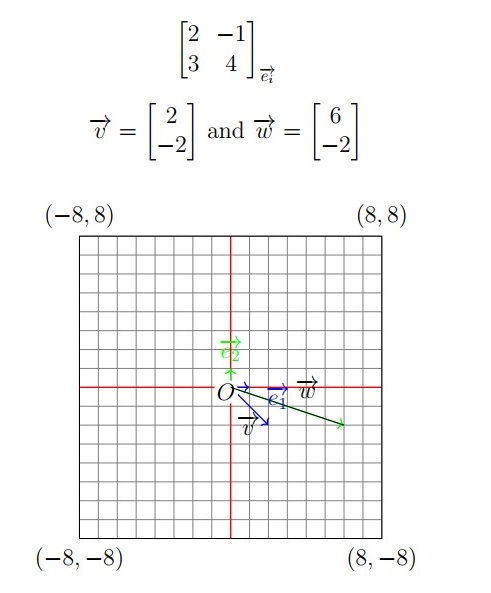
\includegraphics[scale=0.75]{5.jpg}
			\label{f5}
		\end{center}
	\end{figure}

	\item Linear Maps(geometrically) are spatial transforms that
	\begin{enumerate}
		\item keep gridlines parallel.
		\item keep gridlines evenly spaced
		\item keep the origin stationary
	\end{enumerate}
		\begin{figure}[htbp]
			\begin{center}
				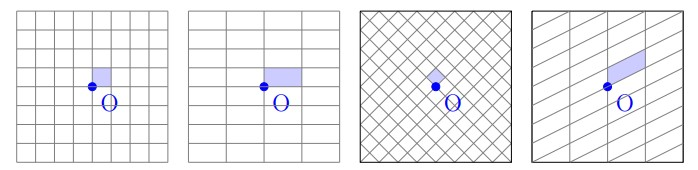
\includegraphics[scale=0.85]{6.jpg}
				\label{f5}
			\end{center}
		\end{figure}
	
	A linear map/linear transformation/vector space homomorphism/linear function is a mapping $v \to w$ between two vector spaces that preserves the operation of vector addition and scalar multiplication.
	
	\begin{figure}[htbp]
		\begin{center}
			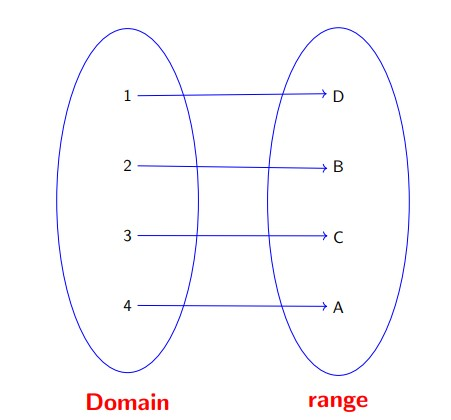
\includegraphics[scale=0.75]{7.jpg}
			\label{f5}
		\end{center}
	\end{figure}
	
	\textbf{Bijection}:A bijection/bijective function/one-to-one correspondence or invertible function, is a function between the elements of two sets, where each element of one set is paired with exactly one element of the other set, and each element of the other set is paired with exactly
	one element of the first set.
	
	If a linear map is a bijection then it is called a linear isomorphism. If \textbf{V} = \textbf{W} then the linear map is called endomorphism(input vector space is identical to output vector space).
	
	\item Linear map (abstractly) follows
	\begin{itemize}
		\item  Maps vectors to vectors $L:V\to W$
		\item Add inputs or the output $L(\overrightarrow{V} + \overrightarrow{W}) = L(\overrightarrow{V}) + L(\overrightarrow{W})$
		\item Scale the inputs then linear mapping or scale output of linear map of input
		$$L(n\overrightarrow{V}) = nL(\overrightarrow{V})$$
	\end{itemize}

	\end{enumerate}

	In old basis, $\overrightarrow{e_{1}},\overrightarrow{e_{2}},\overrightarrow{e_{3}}$ with linear map L and in new basis $\widetilde{\overrightarrow{e_{1}}},\widetilde{\overrightarrow{e_{2}}},\widetilde{\overrightarrow{e_{3}}}$ with linear map $\widetilde{L}$.
	
	\begin{center}
		\begin{align*}
			L(\overrightarrow{e_{1}}) &= L^{1}_{1}\overrightarrow{e_{1}} + L^{2}_{1}\overrightarrow{e_{2}} + L^{3}_{1}\overrightarrow{e_{3}}\\
			L(\overrightarrow{e_{2}}) &= L^{1}_{2}\overrightarrow{e_{1}} + L^{2}_{2}\overrightarrow{e_{2}} + L^{3}_{2}\overrightarrow{e_{3}}\\
			L(\overrightarrow{e_{3}}) &= L^{1}_{3}\overrightarrow{e_{1}} + L^{2}_{3}\overrightarrow{e_{2}} + L^{3}_{3}\overrightarrow{e_{3}}
		\end{align*}
	\end{center}

	\section*{Tensor Product Spaces}
	\begin{tcolorbox}
		\begin{align*}
			& n(\overrightarrow{v}\otimes\alpha) = (n\overrightarrow{v})\otimes\alpha = \overrightarrow{v}\otimes(n\alpha)\\
			& \overrightarrow{v}\otimes\alpha + \overrightarrow{v}\otimes\beta = \overrightarrow{v}\otimes(\alpha + \beta)\\
			& \overrightarrow{v}\otimes\alpha + \overrightarrow{w}\otimes\alpha = (\overrightarrow{v}+\overrightarrow{w})\otimes\alpha
		\end{align*}
	\end{tcolorbox}
	
	Let's say 
	$$\overrightarrow{a}\otimes\overrightarrow{b}\otimes\overrightarrow{v}\otimes\overrightarrow{d}\otimes\overrightarrow{e} + \overrightarrow{a}\otimes\overrightarrow{b}\otimes\overrightarrow{w}\otimes\overrightarrow{d}\otimes\overrightarrow{e} = \overrightarrow{a}\otimes\overrightarrow{b}\otimes(\overrightarrow{v} + \overrightarrow{w})\otimes\overrightarrow{d}\otimes\overrightarrow{e}$$
	
	Such scaling and adding rules refers to vector space.
	\large
	\begin{align*}
		\overrightarrow{v},\overrightarrow{w},\overrightarrow{e_{1}},\overrightarrow{e_{2}}\quad\quad &\in V \quad\text{ these vectors exist in product space V}\\
		\alpha,\beta,\epsilon^{1},\epsilon^{2}\quad\quad &\in V^{*}\quad \text{ these co-vectors exist in dual space}\\
		\overrightarrow{v}\otimes\alpha,\overrightarrow{v}\otimes\beta,\overrightarrow{w}\otimes\alpha,\overrightarrow{w}\otimes\beta,\overrightarrow{e_{1}}\otimes\epsilon^{2},L^{i}_{j}\overrightarrow{e_{i}}\otimes\epsilon^{j}\quad\quad &\in V\otimes V^{*}
	\end{align*}
	\Large
	So in the last statement, we can see that vector co-vector pair such  $\overrightarrow{v}\otimes\alpha,\overrightarrow{v}\otimes\beta,\overrightarrow{w}\otimes\alpha$ etc. can be scaled and added. So these belongs to a vector space and that is $V\otimes V^{*}$ since we are combining spaces. 

\end{document}















